% n_s mean: 1.7+/-0.8
% n_p mean: (3+/-9)e+01
% Brewster Winkel: $\alpha_{\text{B}}=75\,°$
% Brechungsindex theorie $n = 3,73$
% Brechungsindex $n_{\text{s}} = \left(1,34\pm 0,12\right)$
% Brechungsindex $n_{\text{p}} = \left(3,6\pm 1,9\right)$
\nocite{anleitungV407}
\section{Auswertung}
\label{sec:Auswertung}
Gemessener Nullstrom $$I_0 = 460\,\unit{\micro\ampere}$$
Gemessener Dunkelstrom $$I_{\text{D}} = 2,8\,\unit{\nano\ampere}$$
\begin{table}[H]
    \centering
    \caption{Gemessene Photoströme bei s- und p-polarisiertem Licht in Abhängigkeit vom Einfallswinkel $\alpha$.}
    \label{tab:gedämpfteSchwingung}
    \begin{tblr}{colspec={c c c|| c c c|| c c c}}
        \toprule
        $\alpha\,[°]$ & $I_{\text{s}}\,[\unit{\micro\ampere}]$ & $I_{\text{p}}\,[\unit{\micro\ampere}]$ & $\alpha\,[°]$ & $I_{\text{s}}\,[\unit{\micro\ampere}]$ & $I_{\text{p}}\,[\unit{\micro\ampere}]$ & $\alpha\,[°]$ & $I_{\text{s}}\,[\unit{\micro\ampere}]$ & $I_{\text{p}}\,[\unit{\micro\ampere}]$ \\
        \midrule  
        6   &   6   &   14  &   38  &   24  &   20  &   70  &   110 &   3   \\
        8   &   8   &   14  &   40  &   31  &   20  &   71  &   120 &   1   \\
        10  &   7   &   15  &   42  &   28  &   20  &   72  &   120 &   2,2 \\
        12  &   10  &   15  &   44  &   39  &   20  &   73  &   130 &   1,4 \\
        14  &   6   &   14  &   46  &   38  &   20  &   74  &   140 &   0,9 \\
        16  &   11  &   11  &   48  &   47  &   20  &   75  &   140 &   0,5 \\
        18  &   10  &   16  &   50  &   46  &   20  &   76  &   130 &   0,57\\
        20  &   10  &   16  &   52  &   55  &   19  &   77  &   150 &   0,76\\
        22  &   12  &   16  &   54  &   64  &   17  &   78  &   140 &   1,5 \\
        24  &   15  &   17  &   56  &   70  &   16  &   79  &   160 &   2,8 \\
        26  &   12  &   17  &   58  &   70  &   16  &   80  &   150 &   4,6 \\
        28  &   17  &   18  &   60  &   80  &   14  &   82  &   170 &   10  \\
        30  &   14  &   18  &   62  &   78  &   12  &   84  &   160 &   23  \\
        32  &   19  &   19  &   64  &   90  &   10  &   86  &   190 &   43  \\
        34  &   18  &   19  &   66  &   90  &   8   &   87  &   190 &   60  \\
        36  &   26  &   19  &   68  &   110 &   5   &   &   & \\      
        \bottomrule
    \end{tblr}
  \end{table}

% \begin{figure}
%   \centering
%   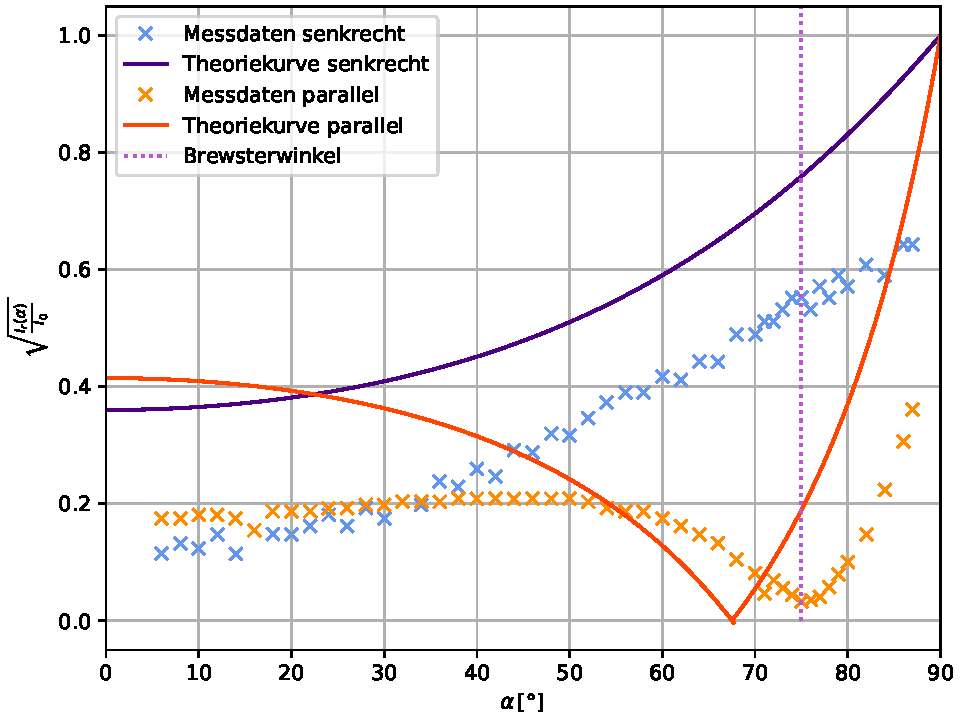
\includegraphics{plot.pdf}
%   \caption{Plot.}
%   \label{fig:plot}
% \end{figure}

%Siehe \autoref{fig:plot}!